%
% $RCSfile$
%
% Copyright (c) 2002-2006. Christian Heller. All rights reserved.
%
% Permission is granted to copy, distribute and/or modify this document
% under the terms of the GNU Free Documentation License, Version 1.1 or
% any later version published by the Free Software Foundation; with no
% Invariant Sections, with no Front-Cover Texts and with no Back-Cover
% Texts. A copy of the license is included in the section entitled
% "GNU Free Documentation License".
%
% http://www.cybop.net
% - Cybernetics Oriented Programming -
%
% http://www.resmedicinae.org
% - Information in Medicine -
%
% Version: $Revision$ $Date$ $Author$
% Authors: Christian Heller <christian.heller@tuxtax.de>
%

\subsubsection{Communication Model}
\label{communication_model_heading}

Systems (alive or not) never communicate directly, but always across the detour
of an external (transient or persistent) \emph{Medium}. This makes it necessary
to use special \emph{Communication Models}, since nearly always, only
\emph{parts} of a complete \emph{Domain Model} want to be exchanged. The use of
communication (transfer) models again, entails the use of model
\emph{Translators}. Sowa \cite{sowa} writes in his book
\emph{Knowledge Representation}:

\begin{quote}
    In computer science, there is no end to the number of specialized notations.
    Besides the hundreds of programming languages, there are diagrams for circuits,
    flowcharts, parse trees, game trees, Petri nets, PERT charts, neural networks,
    design languages, and novel notations that are invented whenever two
    programmers work out ideas at the blackboard. Musical notation \ldots\
    is an example of a complex language that is both precise and human factored.
    As long as the mapping rules are defined, all of these notations can be
    automatically translated to or from logic.
\end{quote}

Although he does not talk of \emph{Domain-} and \emph{Communication Models},
but of \emph{Notations}, Sowa obviously means the same: Any kind of abstract
model can be translated into any other kind, as long as the translation
\emph{Rules} are defined. Model \emph{Translators} are able to map domain model
data to transfer model data. Depending on which communication style is used,
different translators with different rules need to be applied.

\begin{figure}[ht]
    \begin{center}
        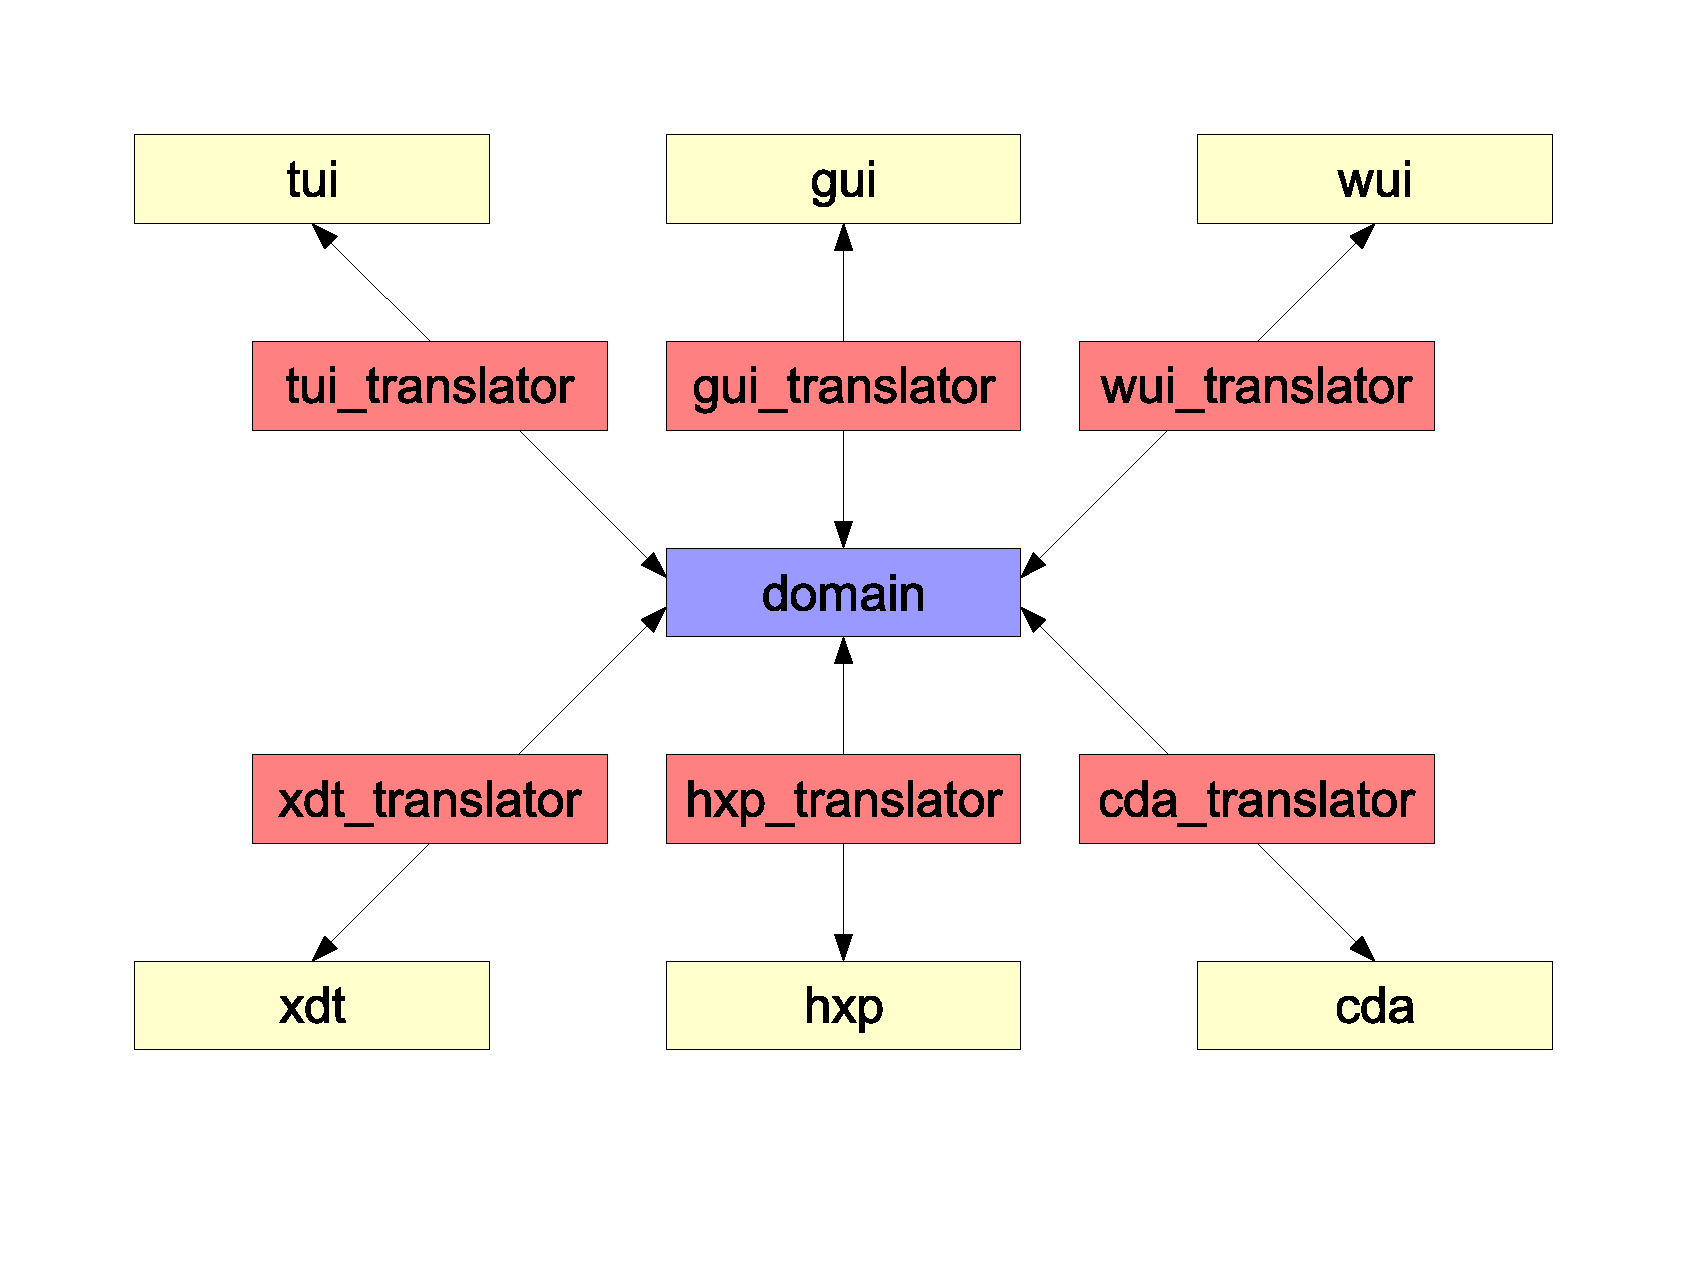
\includegraphics[scale=0.2]{vector/translators.eps}
        \caption{Different Model Translators}
        \label{translators_figure}
    \end{center}
\end{figure}

Figure \ref{translators_figure} shows a number of possible model translators,
for a: \emph{Textual User Interface} (TUI), \emph{Graphical User Interface}
(GUI) and \emph{Web User Interface} (WUI) as well as for the German standard
file format for exchanging medical data called \emph{x Daten Tr\"ager} (xDT),
the \emph{Healthcare Xchange Protocol} (HXP) and \emph{Health Level Seven}
(HL7)'s exchange format called \emph{Clinical Document Architecture} (CDA).

Many application systems have exactly one domain model but transfer models of
arbitrary type should be addable anytime. Translators only know how to
translate between the domain model and a special transfer model, of course in
both directions. \emph{Direct} translation between transfer models is an
exception; it is possible but better done \emph{via} the domain model.

The type of transfer model is independent from the communication mechanism
used. The usage of a \emph{Graphical User Interface} (GUI) model, for example,
is not necessarily limited to human-computer interaction. It could very well be
used for data transfer between remote computers, as long as both systems know
how to translate that model.
